\documentclass[a4paper,14pt]{extarticle}
\usepackage{../../tex-shared/report-layout}

\renewcommand{\mylabnumber}{5}
\renewcommand{\mylabtitle}{Линейный дискриминантный анализ. Построение
канонических и классификационных функций}
\renewcommand{\mysubject}{Интеллектуальный анализ данных}
\renewcommand{\mylecturer}{Сырых О.А.}

\begin{document}
\begin{titlepage}
    
    \thispagestyle{empty}
    
    \begin{center}
        
        Министерство науки и Высшего образования Российской Федерации \\
        Севастопольский государственный университет \\
        Кафедра ИС
        
        \vfill

        Отчет \\
        по лабораторной работе №\mylabnumber \\
        \enquote{\mylabtitle} \\
        по дисциплине \\
        \enquote{\MakeTextUppercase{\mysubject}}

    \end{center}

    \vspace{1cm}

    \noindent\hspace{7.5cm} Выполнил студент группы ИС/б-17-2-о \\
    \null\hspace{7.5cm} Горбенко К. Н. \\
    \null\hspace{7.5cm} Проверил \\
    \null\hspace{7.5cm} \mylecturer

    \vfill

    \begin{center}
        Севастополь \\
        \the\year{}
    \end{center}

\end{titlepage}

\section{Цель работы}
\begin{itemize}
    \item закрепить теоретические знания и приобрести практические навыки в
          проведении дискриминантного анализа по экспериментальным данным;
    \item исследовать возможности языка R для проведения дискриминантного
    анализа.
\end{itemize}

\section{Задание на работу}
\begin{enumerate}
    \item Подготовить данных для дискриминантного анализа. Для проведения
          дискриминантного анализ необходимо разделить исходных данных на 3
          кластера.
    \item Создать тренировочную выборку из исходных данных с известной
          группировкой.
    \item Создать выборку оставшихся данных для последующей проверки
          классификации.
    \item Провести дискриминантный анализ по тренировочной выборке используя
          функцию lda().
    \item По полученным данным составить дискриминантную функцию.
    \item Провести классификацию оставшихся данных и построить матрицу
          неточностей.
    \item По полученным результатам сделать выводы.
    \item Провести шаговую процедуру выбора переменных для построения
          дискриминантной модели.
    \item Построить дискриминантную модель с выбранными переменными, составить
          уравнение дискриминантной функции.
    \item Вывести показатели оценки качества построенной модели: матрица
          неточностей, ошибку распознавания, расстояние Махалонобиса.
    \item Сделать выводы по построенной модели. Сравнить полученные результаты с
          моделью в которой использовались все переменные.
    \item Добавить в выборку данные без классификации, используя дискриминантный
          анализ провести классификацию.
\end{enumerate}

\section{Ход работы}
\subsection{Подготовка данных для дискриминантного анализа}
С помощью команды проведем кластерный анализ методом k-средних на 3 кластера:

\begin{lstlisting}
.cluster <-  KMeans(model.matrix(~-1 + health_index + stringency_index, Dataset), centers = 3, iter.max = 10, num.seeds = 10)

Dataset$KMeans <- assignCluster(model.matrix(~-1 + health_index + stringency_index, Dataset), Dataset, .cluster$cluster)
\end{lstlisting}

Получим данные следующего вида (рисунок \ref{fig:data}):

\begin{figure}[H]
    \centering
    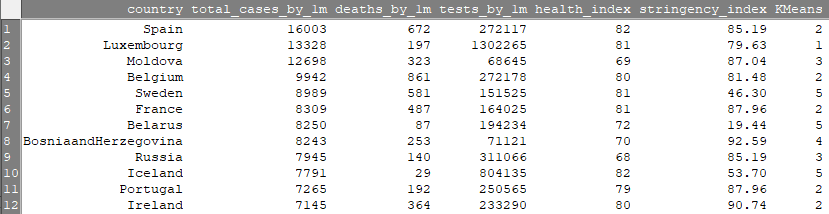
\includegraphics[width=\linewidth]{data}
    \caption{Разбитые на кластеры данные}
    \label{fig:data}
\end{figure}

\subsection{Создание тренировочной выборки}
Создадим выборку строк от 1 до последней с шагом 4:
\begin{lstlisting}
Dataset.train <- Dataset [seq (1, nrow(Dataset),4),]
\end{lstlisting}
Оставшиеся данные сформируем в выборку для последующей проверки полученной классификации:
\begin{lstlisting}
Dataset.unknow <- Dataset [-seq (1, nrow(Dataset),4),]
\end{lstlisting}

\subsection{Проведение дискриминантного анализа}
В качестве переменных используем столбцы 2:6, классификация проводится по столбцу 7:
\begin{lstlisting}
dataset.lda <- lda (Dataset.train[, 2:6], Dataset.train[,7])
\end{lstlisting}

\subsection{Построение дискриминантных функций}
Для построения дискриминантных функций из проведенного анализ используются
Коэффициенты линейных дискриминантов:

\begin{lstlisting}
Coefficients of linear discriminants:
                              LD1             LD2
total_cases_by_1m -0.000139703487 -0.000287021001
deaths_by_1m       0.002212666906  0.001877240490
tests_by_1m       -0.000009048967  0.000004366039
health_index       0.069692377719  0.128238825989
stringency_index  -0.746955798249  0.014550879210
\end{lstlisting}

Получаем две дискриминантные функции:
\begin{enumerate}
    \item $z(x) = -0.747 * stringencyIndex + 0.0697 * healthIndex - 0.000 * \\ * testsBy1m + 0.002 * deathsBy1m - 0.000 * totalCasesBy1m $
    \item $z(x) = 0.015 * stringencyIndex + 0.128 * healthIndex + 0.000 * \\ * testsBy1m + 0.002 * deathsBy1m - 0.000 * totalCasesBy1m$
\end{enumerate}

\subsection{Проведем классификацию и проверку оставшихся данных}
\begin{lstlisting}
> dataset.ldap <- predict(dataset.lda, Dataset.unknow[, 2:6])$class
> dataset.ldap
[1] 1 1 3 1 2 1 3 1 1 3 1 3 1 1 1 1 1 1 3 3 1 3 3 2 1 1 3
Levels: 1 2 3
\end{lstlisting}

Для проверки созданной модели построим матрицу неточностей:

\begin{lstlisting}
> table (dataset.ldap, Dataset.unknow[,7]) 
        
dataset.ldap  1  2  3
            1 15  0  1
            2  0  1  1
            3  1  1  7
\end{lstlisting}

По данной матрице видно, что один объект первого класса попал в 3 группу; один
объект второго класса попал в 3 группу; один объект 3 класса попал в 1 группу;
один объект третьего класса попал во вторую группу.

Ошибка распознавания равна:
\begin{lstlisting}
> Err_S <- mean (Dataset.unknow[,7] != dataset.ldap)
> Err_S
[1] 0.1481481
\end{lstlisting}

Расстояние Махалонобиса:
\begin{lstlisting}
> mahDist <- dist(dataset.lda$means %*% dataset.lda$scaling)
> mahDist
          1         2
2 31.522542          
3  7.282644 24.490570
\end{lstlisting}

\subsection{Пошаговое построение дискриминантной модели}
Проведём шаговую процедуру выбора переменных для построения дискриминантной
модели. Для этого используем функцию stepclass() из пакета klaR. Результат
выполнения этой функции представлен на рисунке \ref{fig:stepclass}.

\begin{figure}[H]
    \centering
    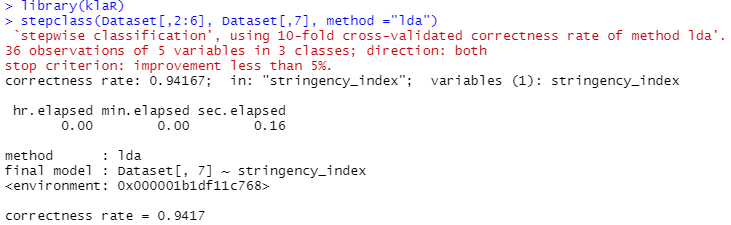
\includegraphics[width=\linewidth]{stepclass}
    \caption{Пошаговое построение дискриминантной модели}
    \label{fig:stepclass}
\end{figure}

Пошаговой процедурой построения модели была выбрана одна переменная -- строгость
реакции властей на пандемию. Для одной переменной невозможно построить
дискриминантную модель.

\subsection{Дискриминантный анализ для данных без классификации}
Добавим в датасет несколько строк без классификации на кластеры (рисунок
\ref{fig:new-records}).

\begin{figure}[H]
    \centering
    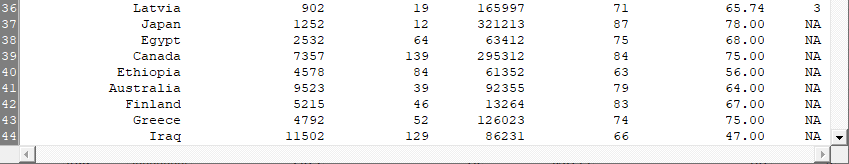
\includegraphics[width=\linewidth]{new-records}
    \caption{Добавленные в датасет записи}
    \label{fig:new-records}
\end{figure}

Выполним дискриминантный анализ только для новых данных:
\begin{lstlisting}
> pred <- predict(dataset.lda, Dataset[37:44,2:6])$class
> pred
[1] 3 3 3 2 3 3 3 2
Levels: 1 2 3
\end{lstlisting}

Из новых 8 записей в 3 группу попали 6 объектов, во вторую -- 2, в первую -- 0.

\section*{Выводы}
В ходе выполнения лабораторной работы была создана тренировочная выборка,
выполнен дискриминантный анализ и проведена классификация, а для ее проверки
была построена матрица неточностей. По полученной матрице видно, что
тренировочная выборка привела к построению гипотезы, согласно которой 4 объекта
попали не в «свою» группу.

Во второй части работы была проведена шаговая процедура выбора переменных для
построения дискриминантной модели с помощью функции stepclass() из пакета klaR.

\end{document}